%!TEX program = xelatex

\documentclass[12pt,a4paper]{article}
\usepackage{xeCJK}
\usepackage{amsmath}
\setmainfont{Times New Roman}
\usepackage{setspace}
\usepackage{caption}
\usepackage{graphicx, subfig}
\usepackage{float}
\usepackage{listings}
\usepackage{booktabs}
\usepackage{setspace}%使用间距宏包
\usepackage{mathtools}
\usepackage{amsfonts}

\begin{document} 
\title{homework7}
	\author{11611118 郭思源}  

\begin{spacing}{1.5}%%行间距变为double-space
\section{Question 1}
        Solve the following problem using graphical analysis.
        \[
            \begin{array}{rrrl}
                \min        &  z = 5x_1 &{} + 7x_2        \\
                \text{s.t.} &      2x_1 &{} + 3x_2 &{} \geq 6  \\
                            &      3x_1 &{} -  x_2 &{} \leq 15 \\
                            &      -x_1 &{} +  x_2 &{} \leq 4  \\
                            &      2x_1 &{} + 5x_2 &{} \leq 27 \\
                \multicolumn{4}{c}{x_i\geq 0,\quad i=1,2}
            \end{array}
        \]
\begin{figure}[htbp]
	\centering
	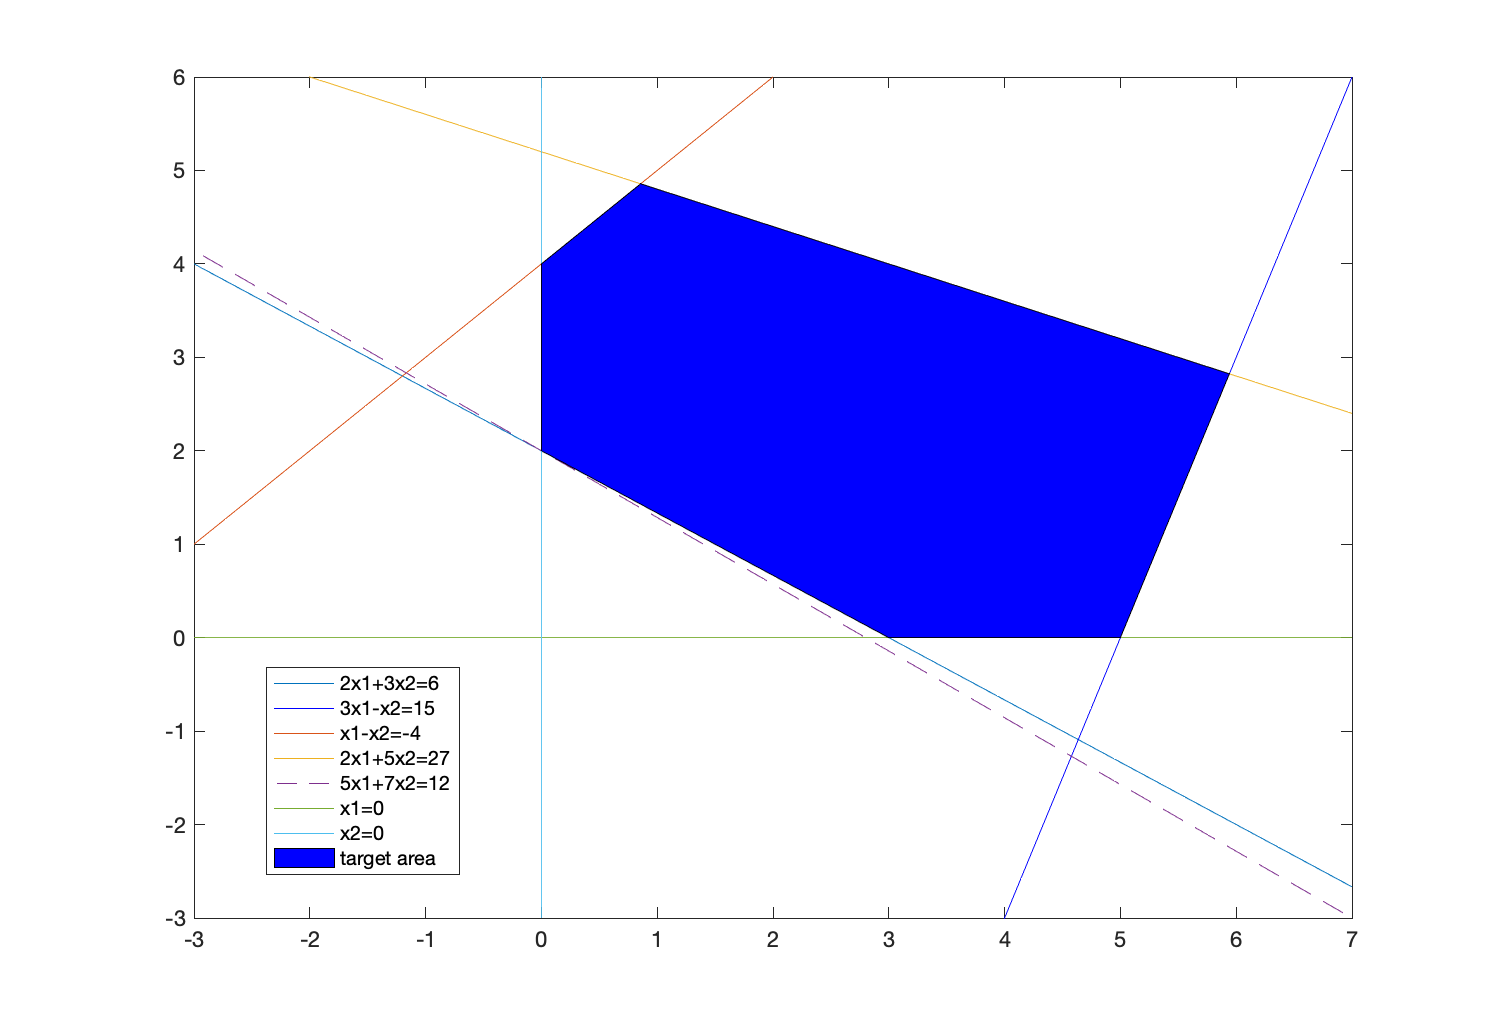
\includegraphics[scale=0.25]{HW7.png}	
\end{figure}

so for min $z=5x_1 +7x_2$ ,we can get at the point$(x_1,x_2)=(0,2)$ 

min $z=5x_1 +7x_2=14$

\end{spacing}


\end{document}